% ch09b_passive_stabilization.tex
% Chapter 9b: Passive Stabilization in Parallel Loops
% "The Physics of Golf" textbook
% Part of the AffineDrift series on golf biomechanics using control-affine decomposition

\chapter{Passive Stabilization in Parallel Loops}
\label{ch:passive_stabilization}

% ============================================================================
% INTRODUCTION
% ============================================================================

\begin{introduction}
  In Chapter~\ref{ch:parallel_mechanisms}, we established that the golf swing is a serial-to-parallel hybrid mechanism: serial segments connected by parallel constraints (the closed kinematic chains formed by the pelvis-torso loop, shoulder girdle closure, and ground contact loop). Those constraints generate forces---the loop Jacobian couples joint motions, the ground reaction forces close the chain, and the X-factor represents an over-constrained constraint on rotation.

  This chapter asks a fundamental question: \emph{Given these constraints, what is the body's stabilization strategy?}

  Intuitively, one might think that tighter muscles (co-contraction) would stabilize the system. Indeed, co-contraction increases joint stiffness and reduces the influence of perturbations. But is this always optimal? Can a \emph{passive} mechanism---pre-tensioned muscles, compliant fascia, favorable geometry---do the stabilization job with less metabolic cost?

  We will see that passive stabilization is not about making the system rigid. Rather, it is about \emph{shaping the potential energy landscape} so that the drift field naturally guides motion toward the desired task. This is Bosch's attractor-fluctuation framework: attractors are low-energy regions where the body can relax into stability; fluctuations are high-energy regions where active control is necessary. A well-tensioned golfer creates favorable attractors throughout the swing; a poorly coordinated golfer must fight against an unfavorable landscape.

  The key insight from affine control theory is that \emph{pre-tensioning modifies the drift field $\drift(x)$, not the control input $\inputmap(x)$}. Thus, passive stabilization is about building a drift field that is already close to the desired trajectory. This is the foundation of Bosch's principle: \emph{Coordinate the assembly lines, not the muscles.}
\end{introduction}

% ============================================================================
% SECTION 1: THE STABILIZATION PROBLEM IN CLOSED KINEMATIC CHAINS
% ============================================================================

\section{The Stabilization Problem in Closed Kinematic Chains}
\label{sec:stabilization_problem}

\subsection{Problem Formulation}

Recall from Chapter~\ref{ch:parallel_mechanisms} that a parallel kinematic chain enforces $m$ loop closure constraints:
\begin{equation}
  \phi_i(\configvec) = 0, \quad i = 1, \ldots, m.
\end{equation}

Each constraint generates a constraint force $\lambda_i$ (a Lagrange multiplier), and the total constraint force is:
\begin{equation}
  \constraintforce = \loopjac^T(\configvec) \boldsymbol{\lambda},
\end{equation}
where $\loopjac(\configvec) \in \Reals^{m \times n}$ is the loop Jacobian and $\boldsymbol{\lambda} \in \Reals^m$ is the vector of constraint multipliers.

The equations of motion become:
\begin{equation}
  \massmat(\configvec) \configddot + \cormat(\configvec, \configdot) \configdot + \gravvec(\configvec) = \boldsymbol{\tau} + \constraintforce.
  \label{eq:constrained_eom}
\end{equation}

\begin{infobox}{In Plain Language}
  This equation says: the net torque on each joint equals (1) the muscle torque $\boldsymbol{\tau}$, (2) constraint forces that keep the kinematic chain closed, plus gravity and Coriolis/centrifugal effects. The constraint forces $\constraintforce$ are not under direct voluntary control; they are \emph{internal} to the mechanism and are determined by the requirement that the chain remain closed.
\end{infobox}

Now comes the stabilization problem: \emph{How should the nervous system manage the constraint forces to maintain task performance in the presence of perturbations?}

There are two competing strategies:

\begin{enumerate}
  \item \textbf{Increase passive stiffness} (co-contraction): Make the joint impedance $\mathcal{Z}(s) = K + D s + M s^2$ large, especially the stiffness $K$. This directly opposes perturbations and reduces the sensitivity of motion to disturbances. The constraint forces are then ``absorbed'' by the stiff joints.

  \item \textbf{Reduce the impact of constraints} (compliance): Keep joints compliant but shape the potential energy landscape so that attractors naturally guide the system toward the desired trajectory. The constraint forces act \emph{with} the gravitational and elastic fields, not against them.
\end{enumerate}

Both strategies have metabolic costs. Co-contraction is expensive (it produces no external work, only heat). Compliance requires active feedback to reject disturbances. The optimal strategy depends on the task, the perturbation spectrum, and the biomechanical constraints.

\subsection{Impedance Control Framework}

Let's formalize the first strategy. In impedance control, a joint is modeled as having target stiffness $K$ and damping $D$:
\begin{equation}
  \boldsymbol{\tau} = K (\configvec_d - \configvec) + D (\configdot_d - \configdot) + \boldsymbol{\tau}_g(\configvec),
  \label{eq:impedance_control}
\end{equation}
where $\configvec_d, \configdot_d$ are the desired position and velocity, and $\boldsymbol{\tau}_g$ is the gravity compensation term.

\begin{infobox}{In Plain Language}
  This says: the muscle produces a torque proportional to the error (desired position minus actual position), plus a damping term proportional to velocity error, plus a term to cancel gravity. This is the classic proportional-derivative (PD) controller. In the musculoskeletal system, stiffness $K$ arises from the intrinsic elasticity of muscle and tendon (passive properties) plus the reflex gains (active feedback). Damping $D$ arises from viscous properties of muscle and reflex delays.
\end{infobox}

The effective impedance matrix $\mathcal{Z}_\text{eff}$ combines the intrinsic joint stiffness (from muscle-tendon elasticity), reflex stiffness (from proprioceptive feedback), and the mechanical coupling through the constraint forces. For a parallel mechanism, the effective impedance seen at the end-effector is:
\begin{equation}
  \mathcal{Z}_\text{eff} = \jacobian^T \mathcal{Z}_\text{joint} \jacobian + \text{(constraint terms)}.
  \label{eq:effective_impedance}
\end{equation}

The problem is that in a parallel mechanism, the constraint terms can \emph{increase} the effective impedance unpredictably. If the constraint forces are large and misaligned with the task direction, they can amplify perturbations or force the system into undesired configurations.

\subsection{Visualization: The Energy Landscape}

A more intuitive way to think about stabilization is through the potential energy landscape $V(\configvec)$. For a conservative system (gravity + elastic potential):
\begin{equation}
  V(\configvec) = m g h(\configvec) + \frac{1}{2} \configvec^T K(\configvec) \configvec + \text{(constraint potential)}.
\end{equation}

An \emph{attractor} is a point $\configvec^*$ where $\nabla V(\configvec^*) = 0$ and the Hessian $H = \nabla^2 V$ is positive-definite (a local minimum). Near an attractor, the system is passively stable: small perturbations produce restoring forces. A \emph{fluctuation} is a region where $V$ is nearly flat (small gradients), so the system does not experience strong restoring forces and must rely on active control.

\begin{figure}[h]
  \centering
  \begin{tikzpicture}[scale=1.0]
    % Axes
    \draw[->, thick] (-0.5, 0) -- (10, 0) node[right] {Joint Angle $\theta$};
    \draw[->, thick] (0, -0.5) -- (0, 6) node[above] {Potential Energy $V(\theta)$};

    % Energy landscape: two attractors separated by a fluctuation region
    % Left attractor (Address position)
    \draw[blue, thick, domain=-0.5:2.5] plot (\x, {(\x - 1)^2 + 0.5});

    % Flat region (fluctuation zone during backswing)
    \draw[green, thick, domain=2.5:5.5] plot (\x, {2.5});

    % Right attractor (Top of swing)
    \draw[red, thick, domain=5.5:10] plot (\x, {(\x - 7)^2 + 0.5});

    % Labels
    \node[blue, below] at (1, 0.5) {Address};
    \node[green, below] at (4, 3) {Fluctuation};
    \node[red, below] at (7, 0.5) {Top};

    % Wells
    \fill[blue, opacity=0.1, domain=-0.5:2.5] (1, 0.5) circle (0.3);
    \fill[red, opacity=0.1, domain=5.5:10] (7, 0.5) circle (0.3);

    % Annotations
    \draw[dashed, gray] (1, 0) -- (1, 0.5);
    \draw[dashed, gray] (7, 0) -- (7, 0.5);
  \end{tikzpicture}
  \caption{Attractor-Fluctuation Energy Landscape. The body begins in a stable well at the address position (blue attractor). During the backswing, the body moves through a flat region (green) where external work must be performed. At the top of the swing, a new attractor forms (red). This shapes the stabilization strategy: the address attractor requires only moderate co-contraction to stabilize; the fluctuation region requires active control; the top attractor uses pre-tension to hold position.}
  \label{fig:energy_landscape}
\end{figure}

% ============================================================================
% SECTION 2: PASSIVE STABILITY THROUGH PRE-TENSIONING
% ============================================================================

\section{Passive Stability Through Pre-Tensioning}
\label{sec:pretensioning}

\subsection{Co-Contraction as a Degrees-of-Freedom Reduction Strategy}

In Bosch's framework (\cite{Bosch2020}), co-contraction is not primarily about stability---it is about \emph{reducing the effective degrees of freedom (DOF)} of the system. When opposing muscles contract simultaneously, they reduce the bandwidth of possible motions, effectively constraining the joint to move along a preferred direction.

Mathematically, suppose a joint has two muscles: an agonist (primary mover) and an antagonist (opposing muscle). The joint torque is:
\begin{equation}
  \tau_j = F_{\text{ago}} r_{\text{ago}} - F_{\text{ant}} r_{\text{ant}},
\end{equation}
where $F$ is muscle force and $r$ is moment arm. If only the agonist contracts, the net torque is unconstrained. But if both contract with forces $F_{\text{ago}}$ and $F_{\text{ant}}$ adjusted so that their average force is held constant while only their \emph{difference} drives motion, the system enters a low-impedance mode.

More formally, in the frame of the constraint forces, co-contraction modifies the effective stiffness matrix:
\begin{equation}
  K_\text{eff} = K_0 + \Delta K_{\text{cocontraction}},
\end{equation}
where $K_0$ is the baseline intrinsic stiffness (from elasticity) and $\Delta K_{\text{cocontraction}}$ is the added stiffness from reflex feedback. The total stiffness can be written in terms of the co-contraction level $\alpha \in [0, 1]$:
\begin{equation}
  K_\text{eff}(\alpha) = (1 - \alpha) K_0 + \alpha K_{\text{max}},
  \label{eq:cocontraction_stiffness}
\end{equation}
where $K_{\text{max}}$ is the maximum achievable stiffness (when agonist and antagonist are fully co-contracted).

\begin{principle}{Co-Contraction Modulates Impedance}
  Co-contraction is a motor strategy to adjust the stiffness of a joint without changing the target position or velocity. By simultaneously contracting opposing muscles, the nervous system can increase the mechanical stiffness of the joint, reducing sensitivity to external perturbations. However, this comes at a metabolic cost: co-contraction produces no external work.
\end{principle}

\subsection{The Viscoelastic Muscle Model: Preflex Control}

The mechanical response of muscle to a sudden length change occurs on a timescale of \SIrange{10}{50}{\milli\second}, which is faster than neural feedback can react (typical reflex latency is \SIrange{50}{100}{\milli\second}). This \emph{preflex} or zero-delay response arises from the passive elastic properties of muscle and tendon.

A simple viscoelastic model of muscle is:
\begin{equation}
  F(t) = K_m \left[ L(t) - L_0 \right] + D_m \dot{L}(t) + F_{\text{active}}(t),
  \label{eq:muscle_viscoelastic}
\end{equation}
where $K_m$ is the intrinsic stiffness of muscle, $D_m$ is the viscous damping, $L$ is the muscle length, and $F_{\text{active}}$ is the actively controlled force (determined by neural input).

\begin{infobox}{In Plain Language}
  Equation~\ref{eq:muscle_viscoelastic} says that muscle force has three components: (1) a spring-like term $K_m (L - L_0)$ that resists length changes, (2) a damper-like term $D_m \dot{L}$ that resists the \emph{rate} of length change, and (3) the actively controlled force. The spring and damper respond immediately to length changes, without waiting for the nervous system.
\end{infobox}

The beauty of preflex control is that it provides \emph{instantaneous stabilization}. If a joint is suddenly perturbed (e.g., by ground reaction forces during impact), the elastic properties automatically generate a restoring force. The nervous system can then use slower feedback (reflex) to fine-tune the response.

For a joint with balanced co-contraction, the effective stiffness and damping are approximately:
\begin{equation}
  K_j = n_{\text{ant}} K_m \sin^2(\phi) + n_{\text{ago}} K_m \cos^2(\phi),
\end{equation}
where $\phi$ is the relative angle between agonist and antagonist moment arms, and $n_{\text{ant}}, n_{\text{ago}}$ are the number of antagonist and agonist muscles. With balanced co-contraction, $K_j$ increases, providing passive stiffness.

\subsection{Force-Length and Force-Velocity Relationships as Passive Stabilizers}

The force-length relationship of muscle (the ascending and descending limbs of the tension curve) and the force-velocity relationship (the hyperbolic relationship between force and shortening velocity) are inherent mechanical properties that do not require active neural control. They automatically stabilize the system:

\begin{enumerate}
  \item \textbf{Force-Length Stability}: If a muscle is stretched beyond its optimal length, passive tension increases (due to titin and collagen in the sarcomere). This resists further stretching. Conversely, if the muscle is shortened below its optimal length, it cannot generate force. This creates a ``zone of comfort'' around the optimal length where stability is highest.

  \item \textbf{Force-Velocity Stability}: The force-velocity relationship means that if the muscle is forcibly lengthened (eccentric contraction), passive tension spikes due to the viscous damping. This opposes the lengthening, providing dynamic stability.
\end{enumerate}

Together, these properties create a \emph{natural attractiveness} to a certain operating range. A well-pre-tensioned joint is one that sits comfortably in the middle of the force-length curve, where small perturbations are automatically resisted.

\subsection{Fascial Pre-Tension and Biotensegrity}

Beyond individual muscles, the fascia (connective tissue surrounding muscles, organs, and entire body regions) can store and distribute elastic potential energy. The biotensegrity model, proposed by Levin and popularized by practitioners of movement, suggests that the body is not a machine of rigid links connected by hinges, but rather a tensioned network where compression elements (bones) are suspended in a web of tension (muscles, fascia, ligaments).

\begin{constraintbox}{Fascial Networks as Passive Stabilization}
  The fascia is not merely a passive wrapper; it is a load-bearing component of the kinetic chain. When pre-tensioned, the fascial network creates a three-dimensional restraint system that distributes loads efficiently and provides passive stabilization without relying on muscular contraction. This is discussed in detail in Chapter~\ref{ch:fascia}.
\end{constraintbox}

Pre-tensioning the fascia (through postural alignment and initial muscle activation) creates a favorable initial condition for motion. Think of it as tuning the strings of a guitar: proper tension distributes loads and allows the whole system to resonate in harmony.

\subsection{Affine Control Interpretation}

From the affine control perspective, pre-tensioning modifies the \emph{drift field}, not the control input. Recall the general form of a control-affine system:
\begin{equation}
  \configdot = \drift(\configvec) + \sum_{i=1}^{m} u_i \inputfield_i(\configvec),
  \label{eq:affine_system}
\end{equation}
where $\drift$ is the drift field (motion under zero input) and $\inputfield_i$ are the control vector fields.

When we pre-tension the system (increase baseline muscle activation or adjust the reference length of antagonist muscles), we change $\drift(\configvec)$. Specifically:
\begin{equation}
  \drift(\configvec) = \drift_0(\configvec) + \Delta \drift_{\text{pretension}}(\configvec),
\end{equation}
where $\Delta \drift_{\text{pretension}}$ represents the change in the natural trajectory caused by the pre-tension. If the pre-tension is well chosen, the new drift field is already oriented toward the desired motion, reducing the need for control inputs.

\begin{driftcontrol}{Pre-Tensioning Optimizes the Drift Field}
  A well-tensioned body has a favorable drift field. The ZTCF (zero-torque counterfactual) trajectory---the motion that would occur if all voluntary control were removed and only passive properties remained---is already close to the intended swing. This is why elite golfers appear to swing effortlessly: their pre-tension creates an attractor that naturally guides the motion.
\end{driftcontrol}

% ============================================================================
% SECTION 3: SELF-ORGANIZATION AND THE ATTRACTOR-FLUCTUATION LANDSCAPE
% ============================================================================

\section{Self-Organization and the Attractor-Fluctuation Landscape}
\label{sec:attractors}

\subsection{Bosch's Attractor-Fluctuation Framework}

Bosch (\cite{Bosch2020}) proposes that human motor control operates by creating energy landscapes with attractors (low-energy regions) and fluctuations (high-energy, unstable regions). The body's primary job is not to compute trajectories but to \emph{structure the landscape} so that motion self-organizes toward the task goal.

In mathematical terms, an attractor is a stable equilibrium of the dynamics. For a system with potential energy $V(\configvec)$, an attractor $\configvec^*$ satisfies:
\begin{equation}
  \nabla V(\configvec^*) = 0, \quad \text{and} \quad \nabla^2 V(\configvec^*) \succ 0.
  \label{eq:attractor_definition}
\end{equation}

The second condition (positive-definite Hessian) ensures local stability: any small perturbation is pushed back toward $\configvec^*$.

By contrast, a fluctuation is a region where $\nabla^2 V$ is nearly singular or has negative eigenvalues. In such regions, the system is marginally stable or unstable, and active control (muscle contraction with feedback) is necessary to maintain the desired trajectory.

\begin{theorem}{Attractor-Driven Stabilization}
  A motor task that involves stable attractors requires less active control and metabolic energy than a task with extensive fluctuation regions. The nervous system designs movement by:
  \begin{enumerate}
    \item Creating attractors at critical task landmarks (e.g., the address position, the top of the swing, the impact point).
    \item Filling fluctuation regions with continuous active feedback to guide the system from attractor to attractor.
    \item Exploiting the passive properties of muscles, tendons, and fascia to maintain attractors without conscious effort.
  \end{enumerate}
  \label{thm:attractor_design}
\end{theorem}

\subsection{Phase Transitions and Control Mode Switching}

As the body moves through a swing, it undergoes phase transitions between different stabilization modes. Early in the backswing, the address attractor is strong: the body is stiff and stable. As the backswing progresses and the golfer builds pre-tension, the old attractor weakens and a new attractor (the top of the swing) forms. At the transition point, the control mode switches: the system transitions from one attractor to another.

This phase transition can be understood mathematically as a bifurcation. The stiffness parameter (controlled by co-contraction level $\alpha$) changes, and the eigenvalues of the linearized dynamics cross the imaginary axis, indicating a loss of stability in one mode and the emergence of stability in another.

\begin{figure}[h]
  \centering
  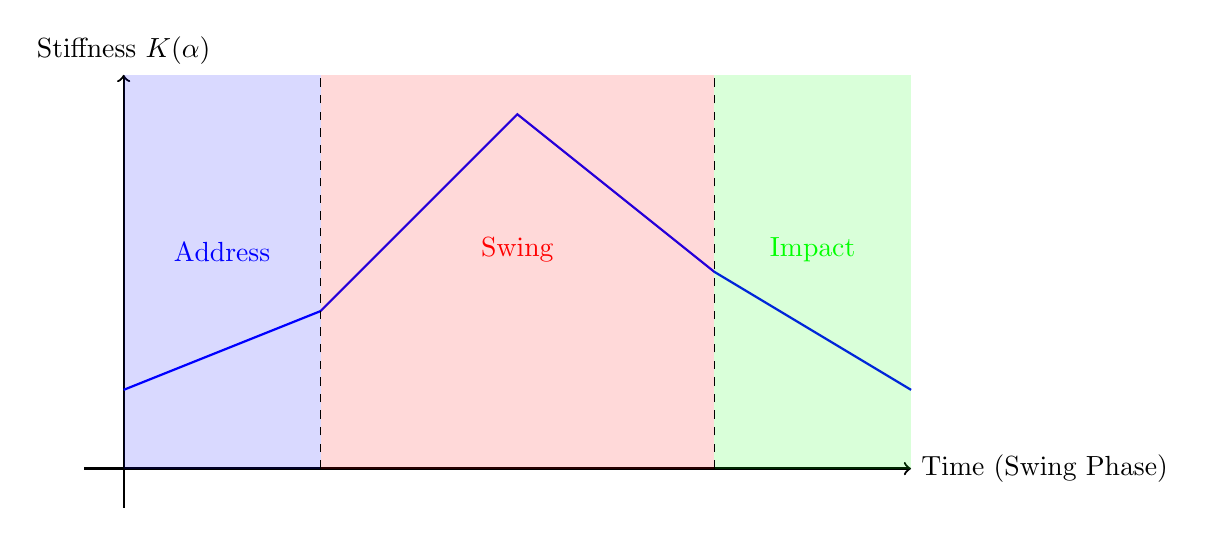
\begin{tikzpicture}[scale=1.0]
    % Coordinate system
    \draw[->, thick] (-0.5, 0) -- (10, 0) node[right] {Time (Swing Phase)};
    \draw[->, thick] (0, -0.5) -- (0, 5) node[above] {Stiffness $K(\alpha)$};

    % Stiffness curve
    \draw[thick, blue] (0, 1) -- (2.5, 2) -- (5, 4.5) -- (7.5, 2.5) -- (10, 1);

    % Phase regions
    \fill[blue, opacity=0.15] (0, 0) -- (2.5, 0) -- (2.5, 5) -- (0, 5) -- cycle;
    \fill[red, opacity=0.15] (2.5, 0) -- (7.5, 0) -- (7.5, 5) -- (2.5, 5) -- cycle;
    \fill[green, opacity=0.15] (7.5, 0) -- (10, 0) -- (10, 5) -- (7.5, 5) -- cycle;

    % Labels
    \node[anchor=south, blue] at (1.25, 2.5) {Address};
    \node[anchor=south, red] at (5, 2.5) {Swing};
    \node[anchor=south, green] at (8.75, 2.5) {Impact};

    % Transition points
    \draw[dashed, black] (2.5, 0) -- (2.5, 5);
    \draw[dashed, black] (7.5, 0) -- (7.5, 5);
  \end{tikzpicture}
  \caption{Phase Transitions in Stiffness During the Golf Swing. The body begins at address with high initial stiffness (blue), maintaining the attractor. During the swing (red), stiffness decreases as pre-tension is transferred to elastic elements (tendons, fascia). At impact (green), stiffness increases again to stabilize the collision forces. The transitions (dashed lines) are critical moments where the control mode switches.}
  \label{fig:phase_transitions}
\end{figure}

\subsection{The Uncontrolled Manifold Hypothesis}

The uncontrolled manifold (UCM) hypothesis, developed by \cite{Scholz1999} and extended by \cite{Schoner2003}, provides an empirical way to test the attractor-fluctuation framework. The hypothesis states that variability in movement is not uniformly distributed across all degrees of freedom. Instead, variance is \emph{concentrated in task-irrelevant directions} (the uncontrolled manifold) and minimized in task-relevant directions.

In terms of the energy landscape, task-relevant directions are those that change the cost function (e.g., the accuracy of the golf shot). Task-irrelevant directions are those where fluctuations do not affect the task. The nervous system tolerates high variance in task-irrelevant directions (allowing self-organization and flexibility) and tightly controls task-relevant directions (maintaining stability where it matters).

Mathematically, if the task cost is $J(\configvec)$, the UCM is defined by:
\begin{equation}
  \text{UCM} = \{ \configvec : \nabla J(\configvec) = \mathbf{0} \}.
\end{equation}

In the subspace perpendicular to the UCM, variance is minimized. This suggests that the attractor is not a point but a \emph{low-dimensional manifold}: the nervous system drives variance into irrelevant dimensions and stabilizes the relevant dimensions.

\subsection{What's Right and What's Overclaimed: The Attractor-Fluctuation Reality}

\begin{mythreality}{``The Body Doesn't Compute Trajectories---It Creates Energy Landscapes''}
  \textbf{What's right:} The body does create energy landscapes (through potential energy, muscle pre-tension, and fascia) that shape motion. Attractors exist and do reduce the need for active control. Variance analysis shows that the nervous system tolerates fluctuations in irrelevant directions.

  \textbf{What's overclaimed:} The claim that ``the body doesn't compute trajectories'' is too strong. The nervous system does maintain internal models and predictions. It does adjust commands based on feedback. The attractor-fluctuation framework is a useful organizing principle, but it is not the complete story. The brain actively shapes both the landscape (via pre-tension) and the control inputs (via feedback). The two work together.

  \textbf{Why it matters for golf:} A golfer must build a favorable energy landscape (through setup, posture, and pre-tension), but this alone does not guarantee a good swing. The golfer must also use active feedback to correct errors and adapt to perturbations. The most efficient swings appear effortless because the attractor is so favorable that active control is minimal---not because there is no control.
\end{mythreality}

% ============================================================================
% SECTION 4: THE DRIFT-CONTROL PERSPECTIVE ON PASSIVE STABILIZATION
% ============================================================================

\section{The Drift-Control Perspective on Passive Stabilization}
\label{sec:drift_control_perspective}

\subsection{Pre-Tensioning Modifies the Drift Field}

Let's formalize the affine control perspective. The golf swing is a control-affine system:
\begin{equation}
  \configdot = \drift(\configvec, \alpha) + \sum_{i=1}^{m} u_i(t) \inputfield_i(\configvec),
  \label{eq:golf_affine}
\end{equation}
where $\alpha$ is the co-contraction level (a parameter that changes slowly), $\configvec$ is the configuration (joint angles, positions), and $u_i(t)$ are the voluntary control inputs (muscle activations above the baseline co-contraction).

The drift field $\drift(\configvec, \alpha)$ includes the effects of gravity, Coriolis forces, centrifugal forces, and the passive properties of muscles and tendons:
\begin{equation}
  \drift(\configvec, \alpha) = -\massmat^{-1}(\configvec) \left[ \cormat(\configvec, \configdot) \configdot + \gravvec(\configvec) - \boldsymbol{\tau}_{\text{passive}}(\configvec, \alpha) \right].
\end{equation}

The key insight is that $\boldsymbol{\tau}_{\text{passive}}(\configvec, \alpha)$ depends on the co-contraction level $\alpha$. Increasing $\alpha$ increases the passive torque, which modifies the drift field. A favorable drift field is one where the ZTCF (zero-torque counterfactual)---the trajectory with $u_i = 0$---is already close to the desired task trajectory.

\subsection{The ZTCF and Task-Specific Adaptation}

The ZTCF is defined as:
\begin{equation}
  \text{ZTCF: } \quad \configdot = \drift(\configvec, \alpha) \quad (\text{with } u_i = 0).
\end{equation}

If the ZTCF is close to the desired trajectory $\configvec_d(t)$, then the control inputs $u_i(t)$ need only make small corrections. This is a key design principle: \emph{let the body's natural dynamics do most of the work}.

Conversely, if the ZTCF is far from the desired trajectory (because the co-contraction is too low or poorly timed), the control inputs must work hard to steer the system. This requires higher metabolic cost and greater reliance on feedback.

Elite golfers are skilled at tuning $\alpha(t)$ throughout the swing to keep the ZTCF favorable. They build pre-tension early (increasing $\alpha$ during setup and backswing), which creates an attractor at the top of the swing. Then, they release the pre-tension at the transition, allowing the drift field to naturally drive the downswing. This is why great golfers appear to swing with minimal muscular effort---because the drift field is doing most of the work.

\subsection{DCR Analysis: How Pre-Tensioning Improves Control Efficacy}

Recall from Chapter~\ref{ch:control_affine_decomposition} the drift-control ratio (DCR):
\begin{equation}
  \text{DCR} = \frac{\|\drift(\configvec)\|^2}{\|\drift(\configvec)\|^2 + \sum_i \|u_i \inputfield_i(\configvec)\|^2}.
\end{equation}

The DCR measures the fraction of the dynamics that is accounted for by the drift field. A high DCR means the drift field is doing most of the work; a low DCR means the control inputs are dominant.

For a well-pre-tensioned system (high $\alpha$), the DCR is higher, because the drift field is richer and closer to the desired trajectory. For a loosely-tensioned system (low $\alpha$), the DCR is lower, because the control inputs must do more work.

\begin{driftcontrol}{Passive Stabilization Through Favorable Drift}
  A well-tensioned body has a favorable drift field---the ZTCF (zero-torque counterfactual) trajectory is already close to the intended swing. This means:
  \begin{enumerate}
    \item The body can reduce the muscle effort required (lower $\|u_i\|^2$).
    \item The system is more robust to delays in feedback (because the drift field is already guiding the right direction).
    \item The motion appears effortless and coordinated, even though significant pre-tension is present.
    \item The DCR is high, indicating that the body's natural dynamics are doing most of the work.
  \end{enumerate}
\end{driftcontrol}

\subsection{Linearization and Stability Analysis}

Near an attractor $\configvec^*$, the dynamics can be linearized:
\begin{equation}
  \delta \configdot = A(\configvec^*) \delta \configvec + B(\configvec^*) \delta u,
\end{equation}
where $A = \frac{\partial \drift}{\partial \configvec}\bigg|_{\configvec^*}$ and $B = [\inputfield_1, \ldots, \inputfield_m]$.

For the attractor to be stable under zero control ($\delta u = 0$), the matrix $A$ must have all eigenvalues in the left half-plane. This requires:
\begin{equation}
  \text{Eigenvalues of } A \text{ have negative real parts.}
\end{equation}

For a simple joint with dominant compliance (springs and dampers), the eigenvalues are related to the natural frequency $\omega_n = \sqrt{K/M}$ and damping ratio $\zeta = D / (2\sqrt{KM})$:
\begin{equation}
  \lambda = -\zeta \omega_n \pm i \sqrt{1 - \zeta^2} \omega_n.
\end{equation}

For stability, both real parts must be negative, which requires $\zeta > 0$ (positive damping) and $K > 0$ (positive stiffness). This justifies the intuition that pre-tensioning (increasing $K$ through co-contraction) stabilizes the system.

% ============================================================================
% SECTION 5: THE COST OF OVER-CONSTRAINT: WHEN STIFFNESS HURTS
% ============================================================================

\section{The Cost of Over-Constraint: When Stiffness Hurts}
\label{sec:overconstraint_costs}

\subsection{Bandwidth Reduction and Loss of Adaptability}

While moderate co-contraction stabilizes the system, excessive co-contraction (over-constraint) reduces the \emph{bandwidth} of movement---the range of frequencies that the system can express. A highly stiffened joint can only respond to slow, low-amplitude perturbations. Fast, high-amplitude perturbations exceed the system's capability, and the joint either breaks (injury) or locks up (loss of smoothness).

Mathematically, the bandwidth is approximately the reciprocal of the response time:
\begin{equation}
  \text{Bandwidth} \approx \frac{\omega_n}{2\pi} = \frac{1}{2\pi}\sqrt{\frac{K}{M}}.
\end{equation}

If we increase $K$ too much (high co-contraction), the bandwidth increases, but so does the stiffness, which makes the system brittle. The system can respond quickly to high-frequency perturbations, but it cannot accommodate slow, large-amplitude deflections (like the ground reaction forces at impact).

\subsection{The Phase Transition Under Loading}

Consider what happens when the system experiences a large external load (e.g., the impact forces at ball strike). The constraint force $\constraintforce$ becomes very large, and the loop closure constraint $\phi(\configvec) = 0$ becomes critical. If the system is over-stiffened, the constraint forces are distributed rigidly across the joints, and the load is borne entirely by the muscles (metabolically expensive) or by structural damage (injury).

If the system is moderately stiffened with good compliance, the load is distributed through multiple DOF, and elastic elements absorb energy (less metabolic cost, less injury risk).

There is a phase transition: as the load increases, the optimal stiffness level decreases. This is captured by the LQR (linear-quadratic regulator) optimality condition:

\subsection{LQR Optimality and the Stiffness-Control Trade-Off}

The optimal control input for a linear system is found by minimizing the cost:
\begin{equation}
  J = \int_0^T \left[ \delta \configvec^T Q \delta \configvec + \delta u^T R \delta u \right] dt,
  \label{eq:lqr_cost}
\end{equation}
where $Q$ penalizes deviation from the desired trajectory and $R$ penalizes control effort (metabolic cost). The solution is a linear feedback:
\begin{equation}
  \delta u^* = -R^{-1} B^T P \delta \configvec,
\end{equation}
where $P$ is the solution to the algebraic Riccati equation.

The key insight is that the optimal control gain depends on the ratio $Q / R$. If $Q$ is large (task error is very costly), the control effort is high. If $R$ is large (metabolic cost is high), the control effort is low. An over-stiffened system effectively increases $R$ (metabolic cost of the co-contraction) without necessarily reducing $Q$ (task error).

\begin{constraintbox}{The Optimal Stiffness is Task and Context Dependent}
  The optimal stiffness is not ``maximum.'' It is tuned to balance:
  \begin{enumerate}
    \item \textbf{Stability requirement}: enough stiffness to maintain the attractor.
    \item \textbf{Bandwidth requirement}: enough compliance to accommodate perturbations.
    \item \textbf{Metabolic cost}: the cost of maintaining co-contraction.
    \item \textbf{Task precision}: the accuracy demanded by the task.
  \end{enumerate}
  Elite golfers tune these factors unconsciously, finding the sweet spot where the swing is both stable and efficient.
\end{constraintbox}

\subsection{Energy Cost and Metabolic Efficiency}

Co-contraction is expensive. When an agonist and antagonist contract simultaneously with forces $F_{\text{ago}}$ and $F_{\text{ant}}$ producing no net joint torque (pure co-contraction), the metabolic cost is:
\begin{equation}
  P_{\text{metabolic}} \propto (F_{\text{ago}} + F_{\text{ant}}) v,
\end{equation}
where $v$ is the contraction velocity. The cost is proportional to the \emph{sum} of forces, not their difference. This is why co-contraction is metabolically expensive: both muscles consume ATP, but neither does useful external work.

During the golf swing, metabolic efficiency is important. A poorly tensioned swing requires high co-contraction throughout, draining energy. A well-tensioned swing minimizes co-contraction by building pre-tension early (when motion is slow and the cost is low) and releasing it strategically.

% ============================================================================
% SECTION 6: STRATEGIES FOR THE GOLF SWING
% ============================================================================

\section{Strategies for the Golf Swing: Applying the Framework}
\label{sec:golf_strategies}

Now let's apply the attractor-fluctuation and drift-control framework to the phases of the golf swing.

\subsection{Phase 1: Setup/Address}

\textbf{Goal}: Establish a stable initial configuration and create a favorable attractor.

\textbf{Strategy}:
\begin{itemize}
  \item Moderate co-contraction ($\alpha \approx 0.4 - 0.6$) to stabilize the stance and spine.
  \item Postural alignment to place the center of mass over the base of support, minimizing the effort needed to maintain balance.
  \item Fascial pre-tension to distribute loads and create a unified structure (biotensegrity).
  \item The energy landscape has a strong attractor at the address position, with positive-definite Hessian.
\end{itemize}

The ZTCF at address should be nearly zero (motion at rest with zero control). This is achieved by careful balance of muscle forces around each joint.

\subsection{Phase 2: Backswing}

\textbf{Goal}: Build elastic potential energy in muscles and tendons while maintaining postural stability.

\textbf{Strategy}:
\begin{itemize}
  \item Progressive increase in co-contraction ($\alpha$ increases from 0.4 to 0.8) as the swing builds speed.
  \item The primary motion is driven by control inputs (voluntary activation), not by drift. The DCR is low.
  \item Pre-tension is stored in elastic elements: the latissimus dorsi is stretched, the posterior shoulder rotators are lengthened, and the spinal erectors are loaded eccentrically.
  \item The old attractor (address) weakens, and a new attractor begins to form at the top of the swing.
\end{itemize}

The backswing is a fluctuation region in the energy landscape. The system is not in a stable well; it is being actively driven uphill, storing energy.

\subsection{Phase 3: Transition (Top of Swing)}

\textbf{Goal}: Switch from active control (backswing) to passive drift (downswing).

\textbf{Strategy}:
\begin{itemize}
  \item Highest co-contraction level ($\alpha \approx 0.9 - 1.0$) to create a strong attractor at the top of the swing.
  \item This locks in the pre-tension: the muscles are loaded, the fascia is tensioned, and the elastic elements are stretched.
  \item A new attractor forms with strong positive-definite Hessian. This is the ``coiled spring'' state.
  \item The downswing will be driven primarily by drift (the elastic recoil), not by new muscle activation. The DCR will be high.
\end{itemize}

This is the critical phase transition. The nervous system switches from actively driving the backswing to passively releasing the elastic energy.

\subsection{Phase 4: Downswing}

\textbf{Goal}: Release elastic energy and drive the club through the ball with minimal muscular effort.

\textbf{Strategy}:
\begin{itemize}
  \item Rapid decrease in co-contraction ($\alpha$ drops from 1.0 to 0.2 - 0.4$) as the muscles relax and allow elastic recoil.
  \item The primary motion is driven by drift: elastic recoil of muscles and tendons, gravity, and Coriolis forces. The DCR is very high.
  \item The attractor at the top of the swing destabilizes and repels the system toward impact position.
  \item The sequence is driven by the proximodistal progression: hip rotation initiates the motion (highest inertia, lowest stiffness), which pulls on the torso, which accelerates the shoulder, which drives the arm, which accelerates the club. Each link is momentarily locked (high stiffness) before passing the motion to the next link.
\end{itemize}

The downswing should feel effortless because the drift field is favorable. The golfer is not ``muscling'' the club; the body is releasing stored energy in a coordinated sequence.

\subsection{Phase 5: Impact and Follow-Through}

\textbf{Goal}: Stabilize the wrist and dissipate impact forces without injury.

\textbf{Strategy}:
\begin{itemize}
  \item Very high co-contraction at the wrist and forearm ($\alpha \approx 0.9$) to absorb the impact forces through the stiffened joints and the elastic properties of muscle.
  \item The ground reaction forces (closing the kinematic loop) are very large at impact. High wrist stiffness is essential to prevent excessive wrist motion and to transmit the force cleanly to the club.
  \item The larger joints (shoulder, hip) can be more relaxed ($\alpha \approx 0.4 - 0.6$) because they are farther from the impact point and experience lower stresses.
  \item Post-impact, the body dissipates energy through controlled deceleration (high damping) and elastic recoil.
\end{itemize}

\subsection{The Assembly Line: Intramuscular to Intermuscular Coordination}

Bosch's concept of ``assembly lines'' in motor coordination refers to the hierarchical structure of muscle activation. Intramuscular coordination is the fine control of motor units \emph{within} a muscle (via the nervous system's ability to recruit and synchronize motor units). Intermuscular coordination is the sequencing of different muscles and muscle groups across joints.

In the golf swing, the assembly line works as follows:

\begin{enumerate}
  \item \textbf{Intramuscular}: Motor units within the hip rotators are recruited progressively, building torque smoothly.
  \item \textbf{Intermuscular}: The hip torque is transmitted to the torso via fascial connections and the spinal muscles, which maintain the X-factor constraint.
  \item \textbf{Intermuscular}: Torso rotation accelerates the shoulder, and shoulder muscles stabilize the scapula while rotators cuff muscles accelerate the humerus.
  \item \textbf{Intermuscular}: Shoulder acceleration pulls on the elbow, and the forearm muscles decelerate the arm while accelerating the club through the wrist.
  \item \textbf{Intramuscular}: At the wrist and forearm, fine intramuscular control ensures a clean impact (smooth force transmission through the club).
\end{enumerate}

This assembly line is optimized for \emph{efficiency and robustness}. Each stage amplifies the motion from the previous stage (proximal to distal), transferring momentum while dissipating little energy. This is the kinetic chain principle, now understood through the lens of affine control and attractor-fluctuation dynamics.

\subsection{The Bosch Attractor Hierarchy}

Bosch identifies a hierarchy of attractors in elite golf:

\begin{enumerate}
  \item \textbf{Attractor 0 (Posture)}: The spine and pelvis maintain a stable, neutral alignment throughout the swing. This is a high-level attractor that constrains all lower-level attractors.

  \item \textbf{Attractor 1 (Hip/Pelvis Rotation)}: The hip rotates around a stable, central axis. The pelvis does not slide forward excessively. This creates a stable reference frame for the upper body.

  \item \textbf{Attractor 2 (X-Factor)}: The relative rotation between pelvis and shoulders is controlled (the X-factor constraint from Chapter~\ref{ch:parallel_mechanisms}). This creates a stable twist in the torso, storing elastic energy.

  \item \textbf{Attractor 3 (Shoulder Rotation)}: The shoulder rotates relative to the pelvis, maintaining the X-factor constraint. The shoulder is a parallel mechanism (multiple muscles supporting the ball-and-socket joint), and the attractor ensures smooth rotation.

  \item \textbf{Attractor 4 (Arm/Wrist Position)}: The arm follows the shoulder rotation, with the wrist in a stable position relative to the forearm. The wrist is minimally flexed or extended, maintaining elastic tension for a clean impact.

  \item \textbf{Attractor 5 (Club Path)}: The club follows a stable path in space, determined by the arm and wrist attractors.
\end{enumerate}

Each attractor is maintained by a combination of pre-tension and active feedback. Disrupting any attractor cascades down the hierarchy: if posture fails, hip rotation becomes unstable, which destabilizes the X-factor, which disrupts shoulder rotation, and so on. This is why Bosch emphasizes the importance of stability at each level.

% ============================================================================
% SECTION 7: EXPERIMENTAL EVIDENCE AND MEASUREMENT
% ============================================================================

\section{Experimental Evidence and Measurement}
\label{sec:experimental_evidence}

\subsection{EMG Studies of Co-Contraction}

Electromyography (EMG) provides a direct window into muscle activation patterns. In elite golfers, EMG recordings during the downswing show a clear pattern:
\begin{enumerate}
  \item \textbf{Backswing}: High, sustained EMG activity in all major muscles (high co-contraction level).
  \item \textbf{Transition}: A brief, sharp increase in EMG amplitude (maximum co-contraction at the top of the swing).
  \item \textbf{Early downswing}: Rapid decrease in EMG activity in most muscles, but sustained activity in proximal muscles (hip rotators) and selective activity in distal muscles (wrist stabilizers).
  \item \textbf{Late downswing}: Minimal EMG activity in most muscles, but high activity in the wrist and forearm just before impact.
  \item \textbf{Impact and follow-through}: High EMG activity in arm and forearm muscles to stabilize the impact; rapid decrease in lower body muscles.
\end{enumerate}

In amateur golfers, the pattern is different: EMG activity is often higher throughout the swing, suggesting persistent co-contraction and higher metabolic cost. The transition is less distinct, indicating a less efficient hand-off between active and passive phases.

\subsection{Variance Analysis and the Uncontrolled Manifold}

Analysis of swing variability can test the attractor-fluctuation hypothesis. If the hypothesis is correct, we expect:
\begin{enumerate}
  \item \textbf{Low variance in task-relevant directions}: The ball-contact point, club head speed, and club path should be highly consistent from swing to swing, even for naturalistic swings.
  \item \textbf{High variance in task-irrelevant directions}: The exact hip angle, shoulder angle, or wrist angle should vary considerably, as long as the task-relevant variables are maintained.
\end{enumerate}

UCM decomposition \cite{Scholz1999} quantifies this by partitioning variance into:
\begin{equation}
  V_{\parallel} = \text{variance in task-relevant directions},
\end{equation}
\begin{equation}
  V_{\perp} = \text{variance in task-irrelevant directions}.
\end{equation}

The hypothesis predicts $V_{\perp} > V_{\parallel}$ in the golf swing. Studies confirm this: elite golfers show much lower variance in club head speed and impact location, but higher variance in joint angles, consistent with self-organization on a low-dimensional attractor.

\subsection{Ground Reaction Force Analysis}

Ground reaction forces (GRF) reveal the constraint forces that close the kinematic loop. During the golf swing, GRF should show:
\begin{enumerate}
  \item \textbf{Address and backswing}: Stable, nearly vertical GRF (weight supported symmetrically).
  \item \textbf{Transition}: Shift of weight toward the front foot, and lateral forces as the body prepares to rotate.
  \item \textbf{Downswing}: Rapid increase in vertical GRF (the ground pushes up on the golfer as the golfer pushes down) and horizontal forces (the golfer pushes laterally to generate rotational torque).
  \item \textbf{Impact}: Transient spike in GRF (the impact force is transmitted through the body to the ground).
  \item \textbf{Follow-through}: Decay of GRF as the swing ends.
\end{enumerate}

The GRF pattern is a fingerprint of how well the golfer is using the ground reaction forces to close the kinematic loop. Elite golfers show smooth, coordinated GRF patterns; amateur golfers often show jerky, asymmetric patterns.

\subsection{Stiffness Estimation from Perturbation Studies}

Joint stiffness can be estimated by applying a small perturbation (force or displacement) to a joint and measuring the restoring force or impedance. For example, a torque pulse can be applied to the ankle, and the ankle's response (position change and restoring torque) is measured. The ratio of restoring torque to position change gives the stiffness.

In the context of the golf swing, such measurements are difficult because the swing is dynamic and transient. However, stiffness can be estimated from steady-state postures (like the address position) and compared between elite and amateur golfers. Studies generally find that elite golfers have higher baseline stiffness at address (due to effective pre-tensioning) but lower stiffness during the swing (allowing for greater compliance and energy absorption).

% ============================================================================
% SECTION 8: ALGORITHMS AND COMPUTATIONAL METHODS
% ============================================================================

\section{Computational Methods: Optimizing the Stiffness Distribution}
\label{sec:optimization}

\begin{algorithm}{Computing Optimal Joint Stiffness Distribution}{alg:stiffness_optimization}
  \textbf{Input:}
  \begin{itemize}
    \item Desired trajectory $\configvec_d(t)$ for a golf swing phase.
    \item Model of joint dynamics, including mass matrix $\massmat(\configvec)$, Coriolis matrix $\cormat(\configvec, \configdot)$, and gravity $\gravvec(\configvec)$.
    \item Muscle model with maximum force $F_{\max,i}$ and moment arms $r_i(\configvec)$ for each joint $i$.
    \item Task cost matrix $Q$ (penalties for trajectory error).
    \item Control cost matrix $R$ (metabolic cost of muscle activation).
    \item Constraint: loop closure constraints $\phi_j(\configvec) = 0$ for $j = 1, \ldots, m$.
  \end{itemize}

  \textbf{Output:} Optimal co-contraction profile $\alpha^*(t)$ and control input profile $u^*(t)$.

  \textbf{Algorithm:}
  \begin{enumerate}
    \item \textbf{Initialize:} Set $\alpha(t) = \alpha_0$ (baseline, e.g., $\alpha_0 = 0.3$).

    \item \textbf{Optimize control inputs:} For the current $\alpha(t)$, solve the LQR problem to find the optimal control inputs $u^*(t)$:
    \begin{equation}
      \min_{u(t)} \int_0^T \left[ (\configvec - \configvec_d)^T Q (\configvec - \configvec_d) + u^T R u \right] dt.
    \end{equation}
    Subject to the dynamics:
    \begin{equation}
      \configdot = \drift(\configvec, \alpha(t)) + \inputmap(\configvec) u(t).
    \end{equation}

    \item \textbf{Evaluate cost:} Compute the total metabolic cost:
    \begin{equation}
      C_{\text{total}} = C_{\text{control}} + C_{\text{cocontraction}},
    \end{equation}
    where $C_{\text{control}} = \int_0^T \|u(t)\|^2_R dt$ (control effort) and $C_{\text{cocontraction}} = \int_0^T w(\alpha(t)) dt$ (metabolic cost of co-contraction, where $w$ is an increasing function).

    \item \textbf{Gradient descent:} Update $\alpha(t)$ using gradient descent:
    \begin{equation}
      \alpha(t) \leftarrow \alpha(t) - \eta \frac{\partial C_{\text{total}}}{\partial \alpha(t)},
    \end{equation}
    where $\eta$ is the step size (learning rate).

    \item \textbf{Iterate:} Repeat steps 2--4 until convergence: $\|\partial C_{\text{total}} / \partial \alpha\|_2 < \epsilon$.

    \item \textbf{Return:} $\alpha^*(t)$ and the corresponding optimal control $u^*(t)$.
  \end{enumerate}

  \textbf{Notes:}
  \begin{itemize}
    \item The key is that increasing $\alpha$ changes the drift field $\drift(\configvec, \alpha)$. A favorable drift field reduces the need for control inputs, thus reducing $C_{\text{control}}$. However, the co-contraction itself has a cost $w(\alpha)$. The algorithm finds the balance.
    \item In practice, this optimization can be solved using dynamic programming (Bellman recursion) or by direct transcription (converting the continuous optimal control problem into a finite-dimensional nonlinear programming problem).
    \item The constraint $\phi_j(\configvec) = 0$ must be satisfied at all times. This can be enforced using penalty methods or Lagrange multipliers.
    \item The output $\alpha^*(t)$ should increase during the backswing (building pre-tension), peak at the top of the swing, and decrease during the downswing (releasing pre-tension). This matches the empirical observations from EMG studies.
  \end{itemize}
\end{algorithm}

\subsection{Practical Computation}

In practice, Algorithm~\ref{alg:stiffness_optimization} is implemented by discretizing time and using numerical optimization. A common approach is direct transcription:

\begin{equation}
  \min_{\configvec_k, u_k, \alpha_k} \sum_{k=1}^{N} \left[ (\configvec_k - \configvec_{d,k})^T Q (\configvec_k - \configvec_{d,k}) + u_k^T R u_k + w(\alpha_k) \Delta t \right]
\end{equation}

subject to:

\begin{equation}
  \configvec_{k+1} = \configvec_k + \Delta t \left[ \drift(\configvec_k, \alpha_k) + \inputmap(\configvec_k) u_k \right]
\end{equation}

\begin{equation}
  \phi_j(\configvec_k) = 0, \quad j = 1, \ldots, m, \quad k = 1, \ldots, N.
\end{equation}

This is a finite-dimensional nonlinear program (NLP) that can be solved using interior-point methods (e.g., IPOPT) or sequential quadratic programming (SQP). The solution gives $\alpha_k^*$ and $u_k^*$ at each time step.

% ============================================================================
% SUMMARY AND KEY TAKEAWAYS
% ============================================================================

\section*{Summary: Passive Stabilization in the Golf Swing}

The central insight of this chapter is that \emph{passive stabilization is not about making the body rigid}. Rather, it is about shaping the energy landscape (through pre-tension, elastic elements, and favorable geometry) so that motion self-organizes toward the task goal.

Key takeaways:

\begin{enumerate}
  \item \textbf{Pre-tensioning modifies the drift field:} By increasing co-contraction, the nervous system changes the natural dynamics of the system. A favorable drift field requires minimal control inputs.

  \item \textbf{Attractors are low-energy regions where stability is passive:} Elite golfers create attractors at critical swing landmarks (address, top of swing, impact). The nervous system maintains these attractors with minimal effort.

  \item \textbf{Optimal stiffness is task dependent:} It is not ``maximum stiffness.'' The optimal strategy balances stability, bandwidth, metabolic cost, and task precision.

  \item \textbf{The assembly line coordinates intramuscular to intermuscular activation:} The kinetic chain works by progressively recruiting muscles in a hierarchical sequence, transferring momentum from proximal to distal.

  \item \textbf{The drift-control ratio (DCR) is the efficiency metric:} A high DCR indicates that the body's natural dynamics are doing most of the work. Elite golfers have high DCR during the downswing (passive release) and lower DCR during the backswing (active building of pre-tension).

  \item \textbf{Experimental evidence supports the framework:} EMG patterns, variance analysis (UCM), and GRF measurements all confirm that elite golfers use passive stabilization effectively.
\end{enumerate}

The practical implication: Improving the golf swing is not about practicing harder (higher control inputs). It is about \emph{building a better landscape}. This means improving posture (to create favorable initial attractors), pre-tensioning strategically (to store elastic energy efficiently), and trusting the body's natural dynamics to drive the swing.

% ============================================================================
% EXERCISES
% ============================================================================

\begin{exercises}{Passive Stabilization in Parallel Loops}

\exercise{1}{Conceptual: Attractor Stability}
Consider a golfer at address. The posture creates an attractor with potential energy $V(\theta) = \frac{1}{2} K \theta^2$, where $\theta$ is a small deviation from ideal posture and $K$ is the ``postural stiffness.''

(a) If $K = 100 \, \text{N\cdot m/rad}$, compute the restoring torque for a deviation of $\theta = 0.05 \, \text{rad}$ (about 3 degrees).

(b) If the torso mass is $m = 30 \, \text{kg}$ and the center of mass is $d = 0.1 \, \text{m}$ from the axis of rotation, what is the gravitational torque due to a forward lean of 0.05 rad?

(c) Is the attractor stable? (Is the postural stiffness sufficient to resist the gravitational torque?)

(d) How much co-contraction is needed to increase $K$ to a level where the attractor is strongly stable (restoring torque is at least 2x the gravitational torque)?

\exercise{2}{Mathematical: Impedance Control}
A golfer's wrist is modeled as a mass-spring-damper system:
\begin{equation}
  M \ddot{\theta} + D \dot{\theta} + K \theta = \tau + \tau_{\text{dist}},
\end{equation}
where $M = 0.02 \, \text{kg\cdot m}^2$ (moment of inertia of the hand and club), $D = 0.5 \, \text{N\cdot m\cdot s/rad}$ (damping), $K$ is the stiffness (variable), $\tau$ is the muscle torque, and $\tau_{\text{dist}}$ is a disturbance (e.g., impact force).

Suppose the muscle uses impedance control: $\tau = K_c (\theta_d - \theta)$, where $\theta_d$ is the desired angle and $K_c$ is the control gain (related to co-contraction level).

(a) Write the closed-loop equation of motion and identify the effective stiffness.

(b) For stability, what is the minimum value of $K_c$ (in units of N\cdot m/rad)?

(c) If $K_c = 100 \, \text{N\cdot m/rad}$, compute the natural frequency $\omega_n$ and damping ratio $\zeta$ of the wrist.

(d) If a disturbance $\tau_{\text{dist}} = 5 \, \text{N\cdot m}$ (impact force) is suddenly applied, what is the steady-state deflection $\theta_{\infty}$? How does it depend on $K_c$?

\exercise{3}{Conceptual: Drift Field and ZTCF}
Consider the golf downswing. The drift field (due to gravity, elastic recoil, and Coriolis forces) points roughly toward the impact position. The control inputs (muscle activation) fine-tune the trajectory.

(a) If the ZTCF (zero-torque counterfactual) is very close to the desired trajectory, is the DCR high or low? What does this mean for muscular effort?

(b) If the ZTCF is far from the desired trajectory (e.g., because pre-tension is inadequate), is the DCR high or low? What is the metabolic cost?

(c) Why do elite golfers appear to swing effortlessly? Explain in terms of the drift field.

\exercise{4}{Computational: Optimize Stiffness During Downswing}
Consider a simplified two-joint model of the golf downswing: hip rotation ($\theta_1$) and shoulder rotation ($\theta_2$). The desired motion is:
\begin{equation}
  \theta_{1,d}(t) = \theta_{1,0} + \frac{\pi}{4} \left[ 1 - \cos\left(\frac{2\pi t}{T}\right) \right],
\end{equation}
\begin{equation}
  \theta_{2,d}(t) = \theta_{2,0} + \frac{\pi}{3} \sin\left(\frac{2\pi t}{T}\right),
\end{equation}
where $T = 0.2 \, \text{s}$ is the downswing duration.

The dynamics are decoupled:
\begin{equation}
  M_i \ddot{\theta}_i + D_i \dot{\theta}_i + K_i(\alpha) \theta_i = \tau_i,
\end{equation}
where $M_1 = 0.5, M_2 = 0.1 \, \text{kg\cdot m}^2$, $D_i = 0.5$ (Ns/rad), and $K_i(\alpha) = K_{0,i} + \alpha \Delta K_i$ with $K_{0,1} = 50, K_{0,2} = 20, \Delta K_1 = 50, \Delta K_2 = 30$ (N\cdot m/rad).

The task cost is $Q = I$ (penalize error equally), and the control cost is $R = I$. The co-contraction cost is $w(\alpha) = 10 \alpha^2$ (quadratic in co-contraction level).

(a) Set up the LQR problem for a fixed $\alpha$. What is the optimal control $u_i^*$ in terms of $\alpha$?

(b) For which values of $\alpha$ (say, $\alpha \in [0, 1]$ discretized in steps of 0.1) is the total cost minimized?

(c) Plot the optimal $\alpha^*(t)$ as a function of time during the downswing. Does it increase or decrease? Why?

(d) Compare the DCR at the optimal $\alpha$ to the DCR at $\alpha = 0$ (no co-contraction) and $\alpha = 1$ (maximum co-contraction). Which is most efficient?

\exercise{5}{Experimental Design: Measuring Stiffness}
Design an experiment to estimate the joint stiffness of the wrist during different phases of the golf swing (address, backswing, top of swing, downswing, impact).

(a) What measurement equipment would you use (force sensors, motion capture, EMG)?

(b) How would you apply a perturbation without disrupting the natural swing?

(c) What are the expected stiffness values (in N\cdot m/rad) at each phase?

(d) How would you compare elite golfers to amateurs based on stiffness measurements?

\exercise{6}{Theoretical: UCM Decomposition}
The uncontrolled manifold (UCM) hypothesis states that variance in irrelevant directions is larger than variance in relevant directions. In the golf swing, the relevant direction is the club head speed at impact (task goal), and irrelevant directions include the exact wrist angle, shoulder angle, etc.

(a) Define the task Jacobian $J_{\text{task}}$ that maps joint angles to club head speed. (You may assume a simple kinematic chain model.)

(b) Define the UCM as the null space of the task Jacobian: $\text{UCM} = \text{null}(J_{\text{task}})$.

(c) If the total variance in joint angle space is $\Sigma$, decompose it into variance within the UCM ($V_{\parallel}$) and variance perpendicular to the UCM ($V_{\perp}$).

(d) The UCM hypothesis predicts $V_{\parallel} > V_{\perp}$. What does this imply about the motor control strategy?

(e) How could you test this hypothesis experimentally?

\end{exercises}

% References for this chapter are managed via the central bibliography in main.tex.
